\section{Durchführung}
\label{sec:Durchführung}

Der Aufbau der Messapparatur ist schematisch in Abbildung \ref{fig:bild1} dargestellt.


\begin{figure}
    \centering
    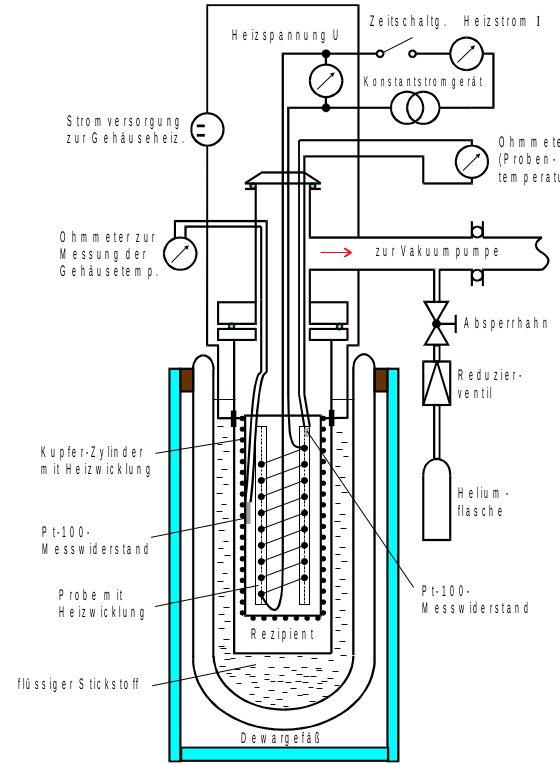
\includegraphics[scale = 0.7]{content/plot2.png}
    \caption{Schematischer Aufbau der Messapparatur [?]}
    \label{fig:bild1}
  \end{figure}


Zunächst wird der Rezipient evakuiert und danach bei Barometerdruckmit Helium gefüllt.
Die Probe wird mithilfe flüssigen Stickstoffs etwa eine Stunde auf $\SI{80}{\kelvin}$ abgekühlt.
Dieser Vorgang wird durch das gut wärmeleitende Helium unterstützt.
Daraufhin wird die Vakuumpumpe eingeschatet, um den Innendruckmöglichst gering zu halten und
mit dem Vakuum die Wärmekonvektion zu verhindern.
Bei der anschließenden Messung wird der Probe über eine Heizwicklung Wärme zugeführt und in 
Temperaturabständen zwischen $\SI{7}{\kelvin}$ und $\SI{11}{\kelvin}$, die über die temperaturabhängigen
 Widerstände von Pt-100-Widerständen gemessen werden, der Heizstrom $I$, die Heizspannung $U$ und die
 Heizdauer $t$ gemessen.
 Durch das Vakkuum und das Halten des Gehäuses auf Stickstofftemperatur, werden Energieverluste durch
 Wärmeleiung, -Strahlung und Konvektion möglichst gering gehalten.

Für Pt-100-Widerstände gilt die Temperatur-Widerstands-Charakteristik

\begin{equation}
    \label{eqn:Temp}
    T = 0.00134 R^2 + 2.296 R - 243.02 \; .
\end{equation}

